\chapter{Bilder}
Für qualitativ hochwertige Dokumente sollten möglichst immer SVG-Grafiken (\url{https://de.wikipedia.org/wiki/Scalable_Vector_Graphics}) bzw. diese als PDF-Dateien verwendet werden. Wenn es Pixelgrafiken (PNG, JPG, TIFF, …) sind, sollte auf eine hohe Auflösung geachtet werden, da besonders im Druck schlechte Auflösungen negativ hervorstechen.

Bilder sollten in die \textit{Fließumgebung} \texttt{figure} gepackt werden. Für Positionierungsoptionen siehe \autoref{sec:fliessumgebungen}. Das Bild innerhalb der Fließumgebung \texttt{figure} wird mit dem Befehl \mintinline{latex}{\includegraphics[options]{path}} durch das Paket \texttt{graphicx} eingefügt. In \texttt{options} sollte immer die Option \mintinline{latex}{width=\columnwidth} gesetzt werden. Bei einem einspaltigen Layout kann alternativ zu \mintinline{latex}{\columnwidth} auch \mintinline{latex}{\textwidth} verwendet werden. Diese Breitenangaben können auch durch Modifikatoren verändert werden. So kann das Bild zum Beispiel auf 80\,\% der Textbreite mit der Option \mintinline{latex}{width=0.8\textwidth} skaliert werden.

\begin{showcase}
    \begin{code}{latex}
        \begin{figure}[Hhtbp] % Here!, here, top, bottom, page
            \centering % ← zentriert das Bild
            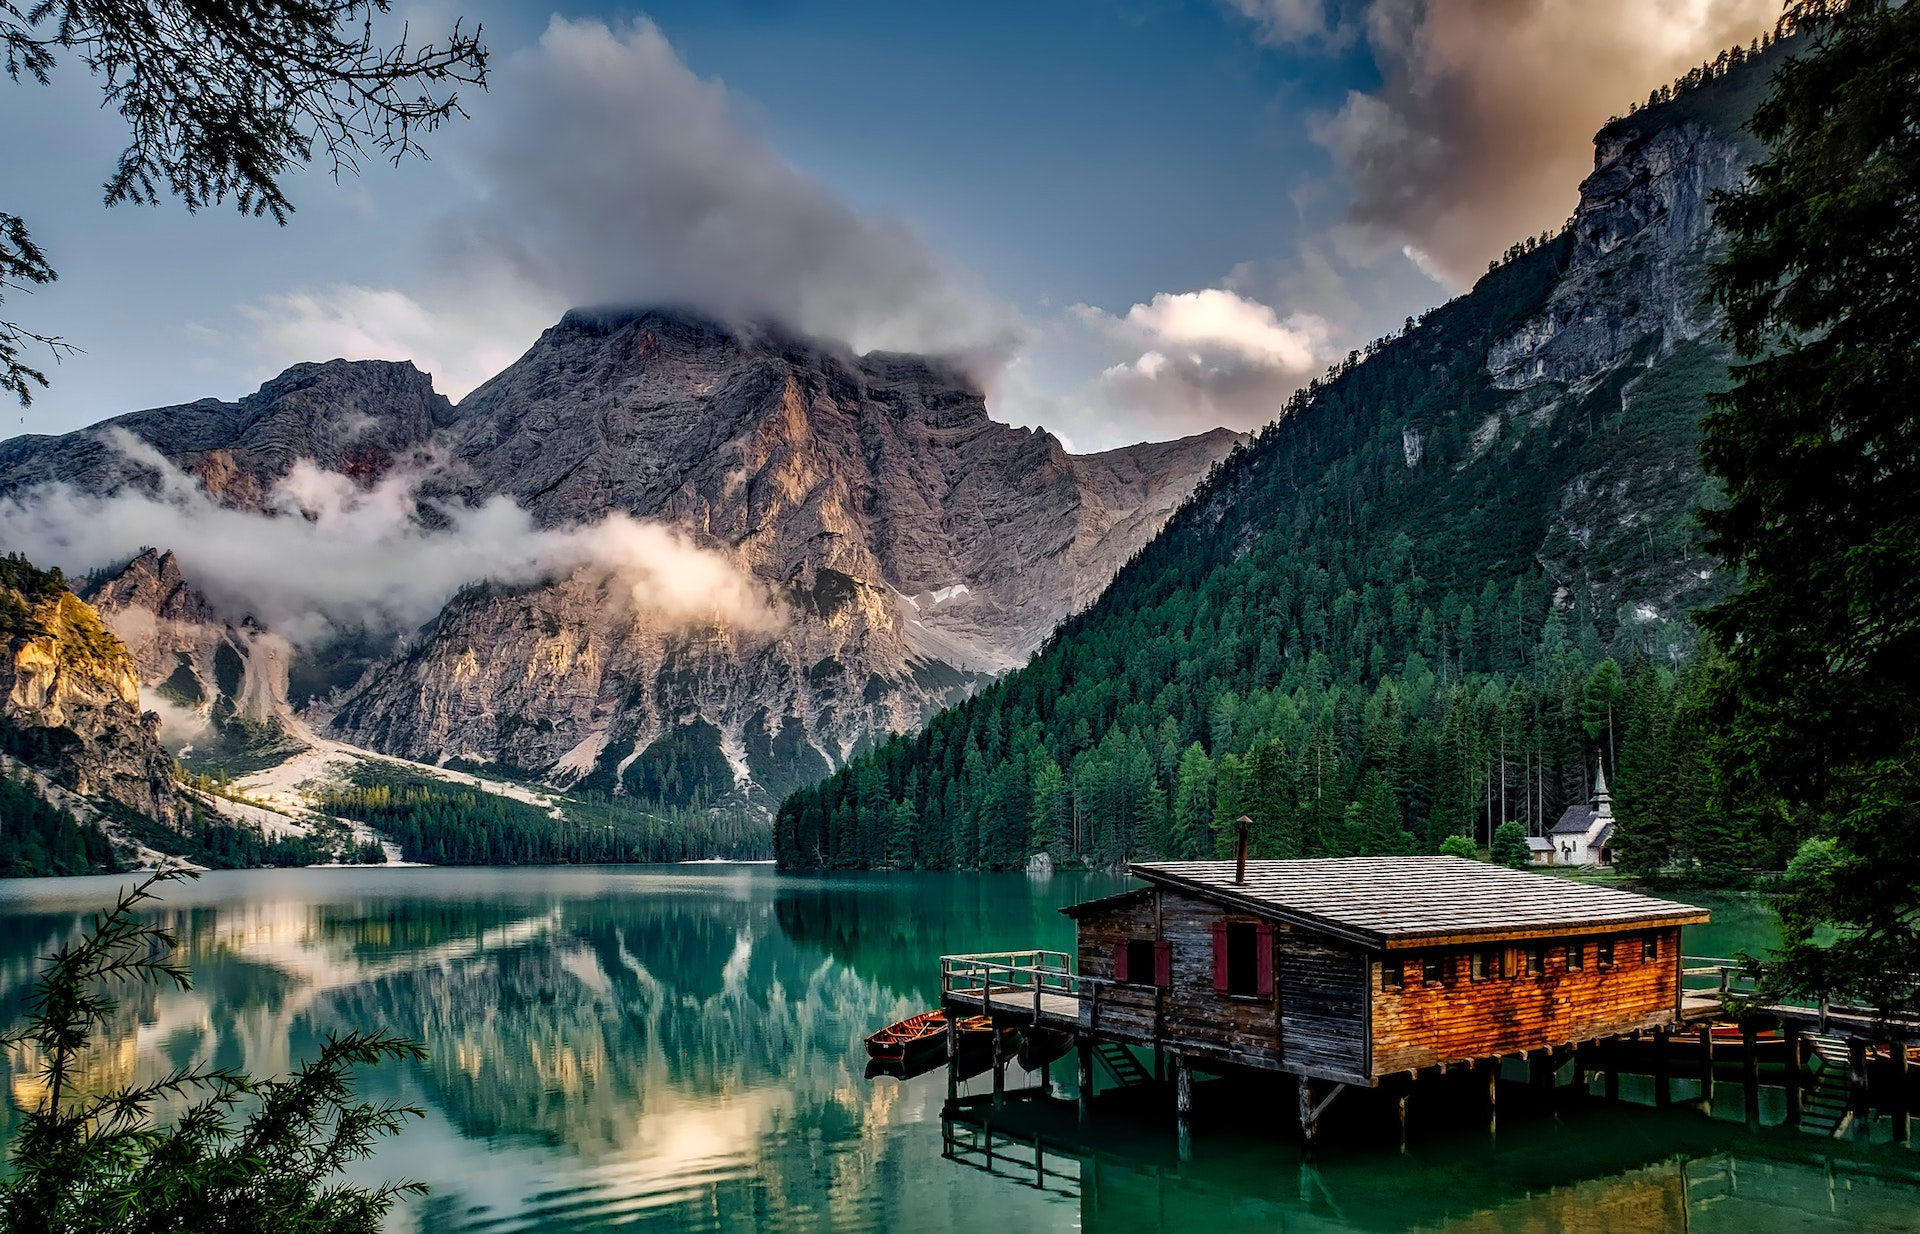
\includegraphics[width=0.8\columnwidth]{assets/images/bilder/pexels-pixabay-147411.jpg}
            \caption{Holzhaus am Gebirgssee}
            \label{fig:holzhaus-am-gebirgssee}
        \end{figure}
    \end{code}
    \tcblower
    \begin{center}
        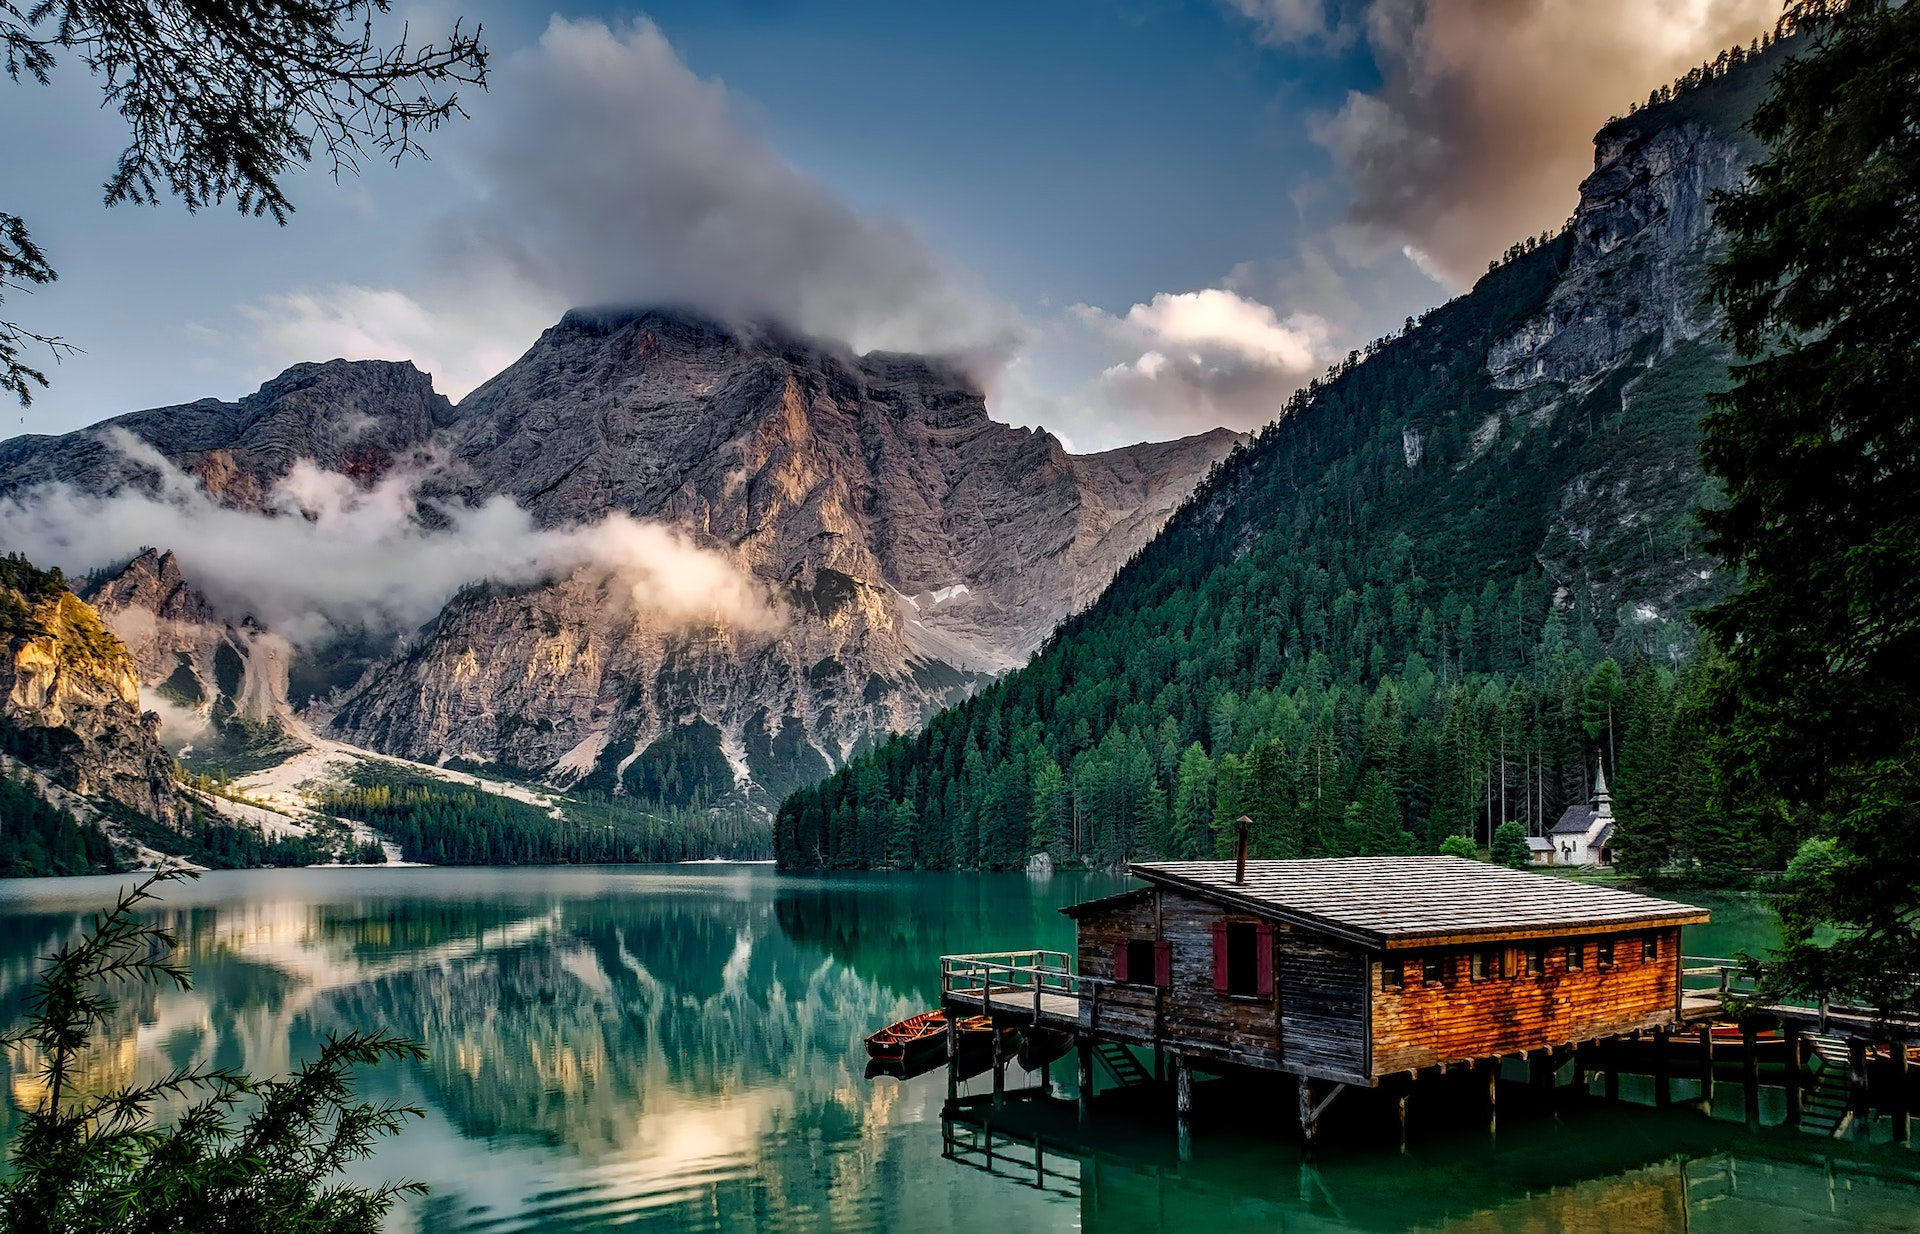
\includegraphics[width=0.8\columnwidth]{assets/images/bilder/pexels-pixabay-147411.jpg}
        \captionof{figure}{Holzhaus am Gebirgssee}
    \end{center}
\end{showcase}

\section{Wrapfigure}
Die \texttt{wrapfigure}-Umgebung in \LaTeX ermöglicht es, Bilder in den Textfluss einzufügen und den umgebenden Text harmonisch um die Abbildung zu positionieren. Im Gegensatz zu herkömmlichen Fließumgebungen, die eine separate Zeile für Abbildungen reservieren, kann \texttt{wrapfigure} das Bild links oder rechts vom Text umfließen lassen. Dies ist besonders nützlich, wenn ein Bild eng mit dem umgebenden Text verbunden ist und eine nahtlose Integration gewünscht ist. Wie in einer normalen Fließumgebung können Beschriftungen mit \mintinline{latex}{\caption{}} gesetzt werden. Die Verwendung von \texttt{wrapfigure}-Umgebung erfordert eine sorgfältige Handhabung, da sie den Textfluss beeinflussen kann. Sie sollte mit Bedacht verwendet werden, um sicherzustellen, dass der Lesefluss und das Layout des Dokuments nicht gestört werden. Für weitere Informationen siehe \url{https://ctan.org/pkg/wrapfig2}.

\begin{table}[H]
    \centering
    \captionabove{Optionen für \texttt{wrapfigure} und \texttt{wraptable}}
    \begin{tblr}{lll}
        \toprule
        \SetCell[c=2]{c}\textbf{Option} & & \textbf{Platzierung} \\
        \midrule
        r & R & rechts, fließend rechts \\
        l & L & links, fließend links \\
        i & I & Innenseite, fließend Innenseite  \\
        o & O & Außenseite, fließend Außenseite \\
        \bottomrule
    \end{tblr}
\end{table}

\begin{showcase}
    …
    \begin{code}{latex}
        \begin{wrapfigure}{r}{0.5\columnwidth}
            \centering
            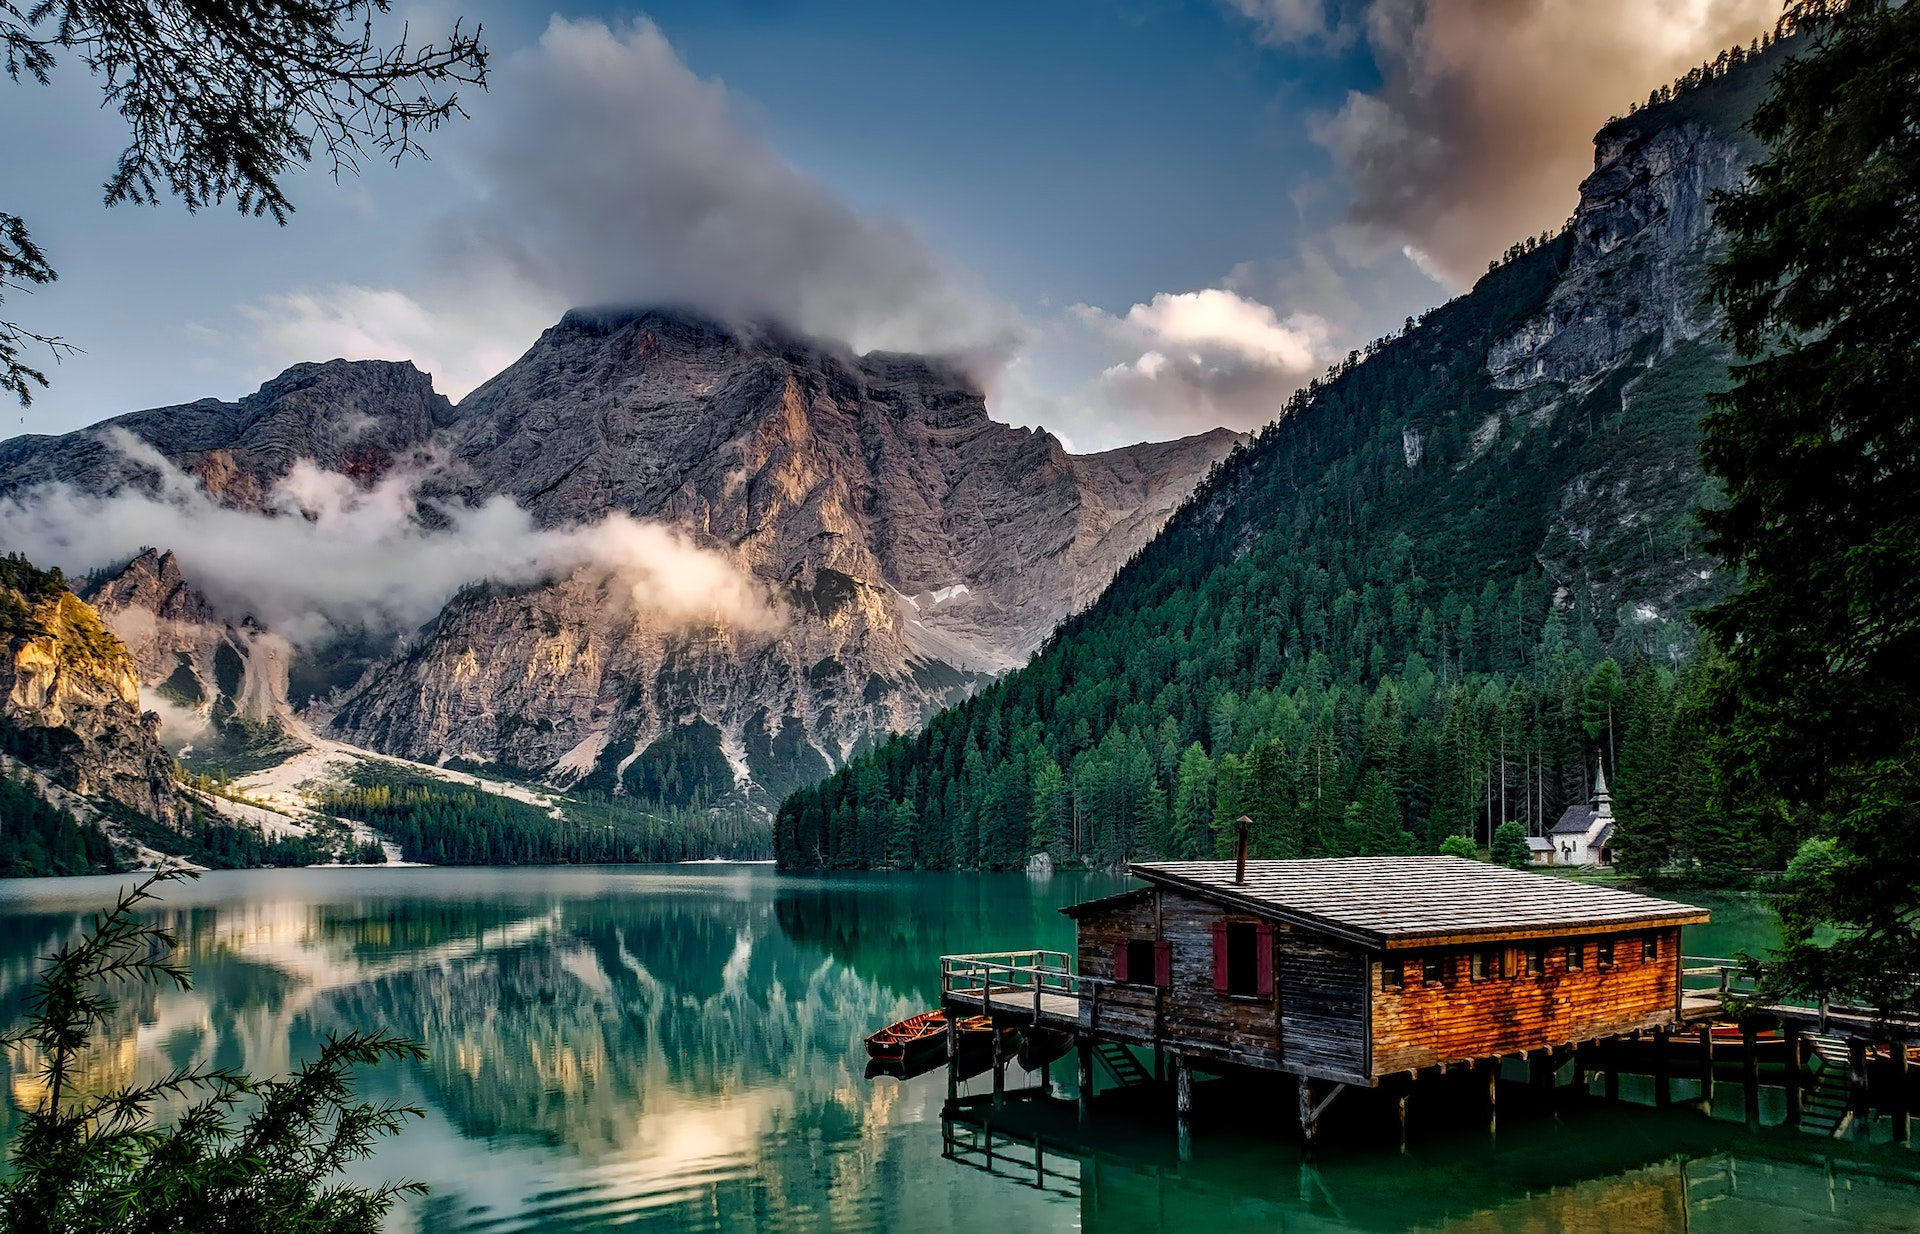
\includegraphics[width=0.5\columnwidth]{assets/images/bilder/pexels-pixabay-147411.jpg}
        \end{wrapfigure}
    \end{code}
    …
    \tcblower
    \begin{wrapfigure}{r}{0.5\columnwidth}
        \centering
        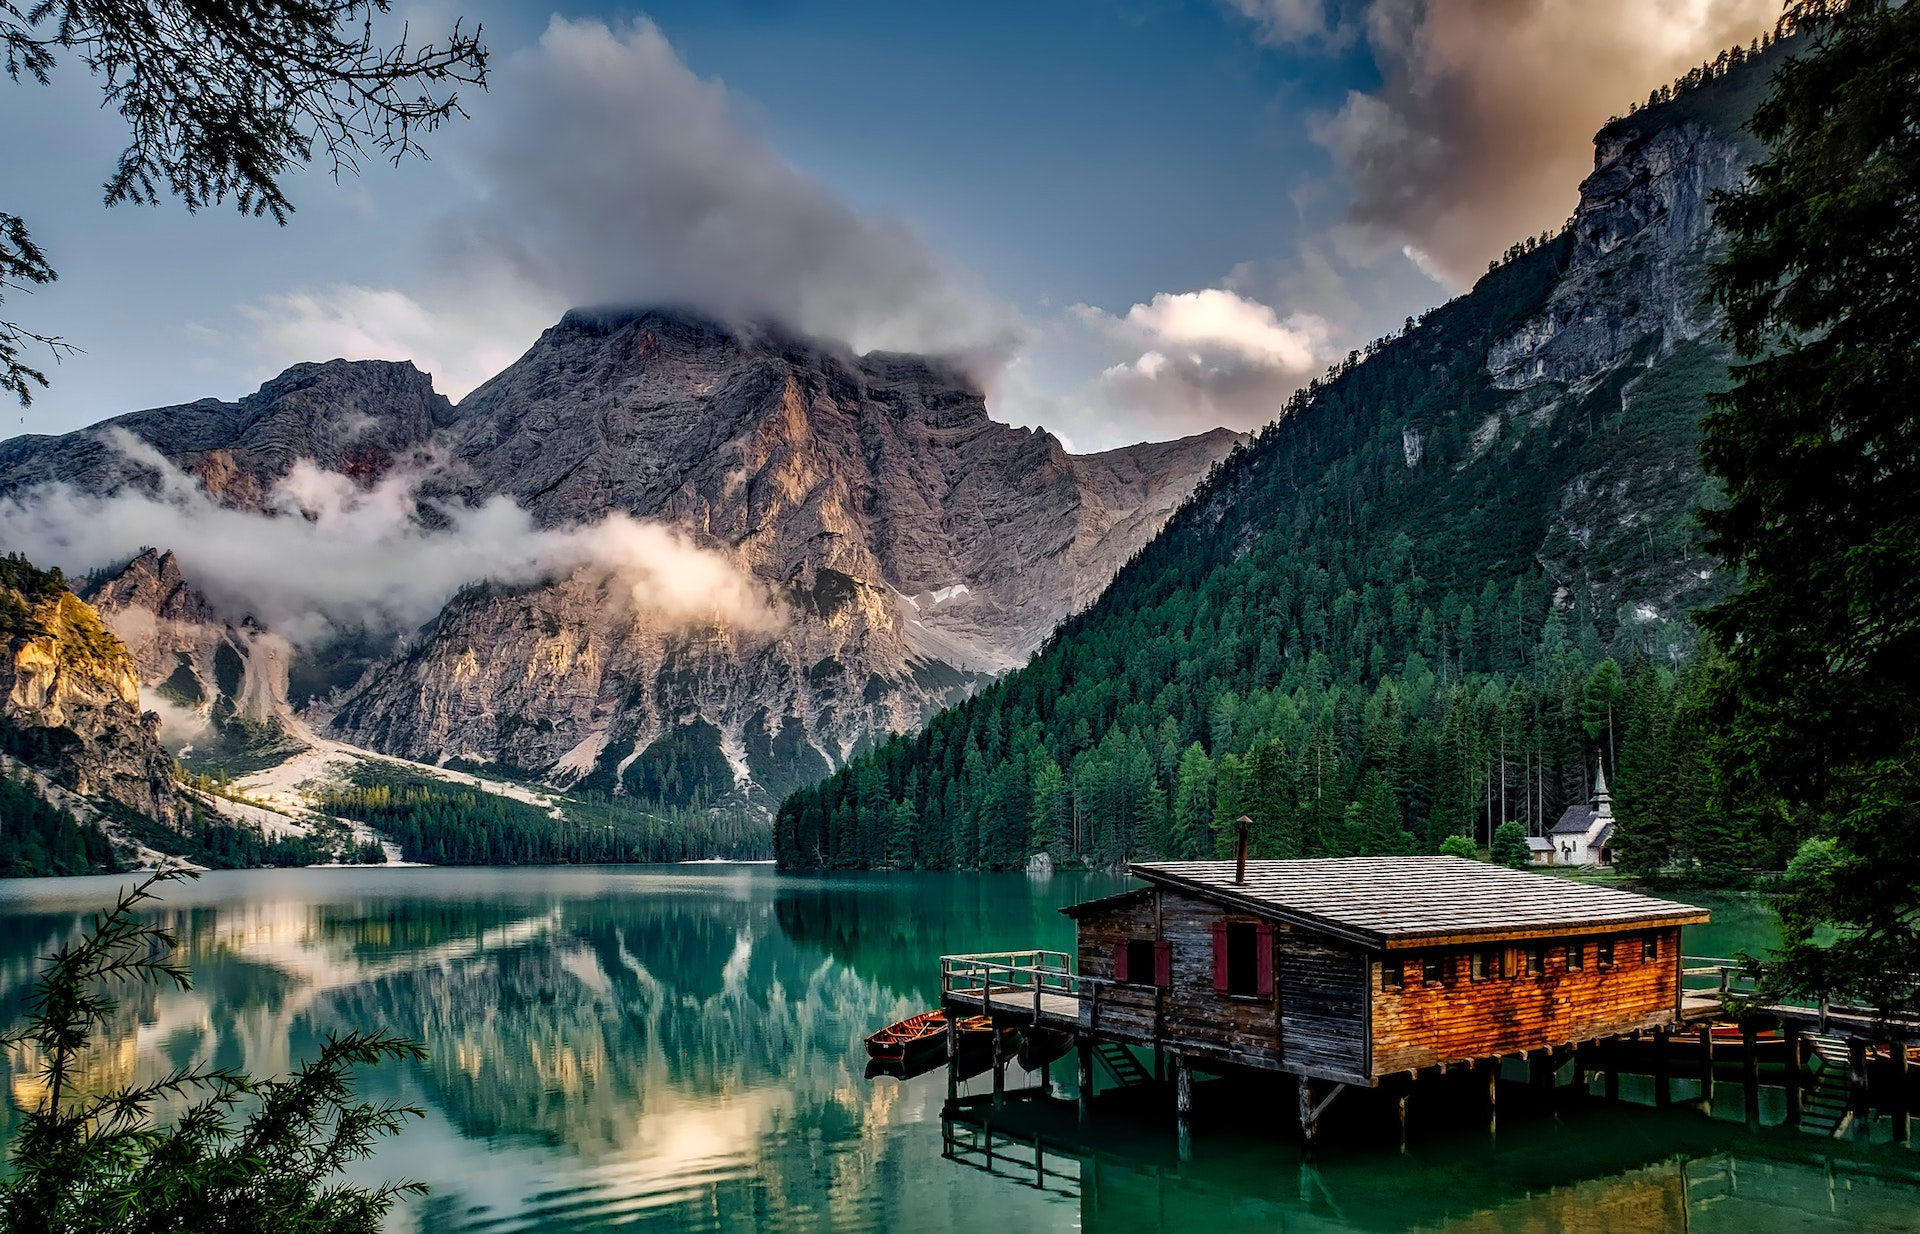
\includegraphics[width=0.5\columnwidth]{assets/images/bilder/pexels-pixabay-147411.jpg}
        \caption{Hütte am See vor dem Kursivgebirge}
    \end{wrapfigure}
    Weit hinten, hinter den Wortbergen, fern der Länder Vokalien und Konsonantien leben die Blindtexte. Abgeschieden wohnen sie in Buchstabhausen an der Küste des Semantik, eines großen Sprachozeans. Nicht einmal von der allmächtigen Interpunktion werden die Blindtexte beherrscht – ein geradezu unorthographisches Leben. Eines Tages aber beschloß eine kleine Zeile Blindtext, ihr Name war Lorem Ipsum, hinaus zu gehen in die weite Grammatik. Der große Oxmox riet ihr davon ab, da es dort wimmele von bösen Kommata, wilden Fragezeichen und hinterhältigen Semikoli, doch das Blindtextchen ließ sich nicht beirren. Es packte seine sieben Versalien, schob sich sein Initial in den Gürtel und machte sich auf den Weg. Als es die ersten Hügel des Kursivgebirges erklommen hatte, warf es einen letzten Blick zurück auf die Skyline seiner Heimatstadt Buchstabhausen, die Headline von Alphabetdorf und die Subline seiner eigenen Straße, der Zeilengasse. Wehmütig lief ihm eine rhetorische Frage über die Wange, dann setzte es seinen Weg fort.
\end{showcase}
